% !TEX root = acsfubAuthorGuidelines-short.tex
\usepackage{tikz}
\usetikzlibrary{positioning,calc}
\usepackage{csquotes}
\usepackage{hyperref}
\usepackage{subfigure}

% ---------------------------------------------------------------------
% EG author guidelines plus sample file for EG publication using LaTeX2e input
% D.Fellner, v2.02, Jan 25, 2017


\title[Generating Spatial Coordinate Datasets from Text Embeddings]%
      {Towards On-Device Continual Learning: A Pipeline for Generating Spatial Coordinate Datasets from Text Embeddings}

% FILMUNI: for anonymous conference submission please enter your SUBMISSION ID
% instead of the author's name (and leave the affiliation blank) !!
% for final version: please provide your *own* ORCID in the brackets following \orcid; see https://orcid.org/ for more details.

% AUTHOR SECTION NOT INCLUDED IN SUBMISSION (BLIND REVIEW)
% \author[P. Gerdes ]
% {\parbox{\textwidth}{\centering P. Gerdes$^{1}$}
% \\
\author[Submission 9]
{\parbox{\textwidth}{\centering Submission 9$^{1}$}
\\
{\parbox{\textwidth}{\centering $^1$Film University Babelsberg KONRAD WOLF, Germany\\} 
}
}

% KEYWORDS (NOT PART OF TEMPLATE):
% Dataset Generation
% Dimensionality Reduction
% Continual Learning

%-------------------------------------------------------------------------
\begin{document}

\teaser{
    \centering
    \subfigure[all-MiniLM-L6-v2 UMAP]{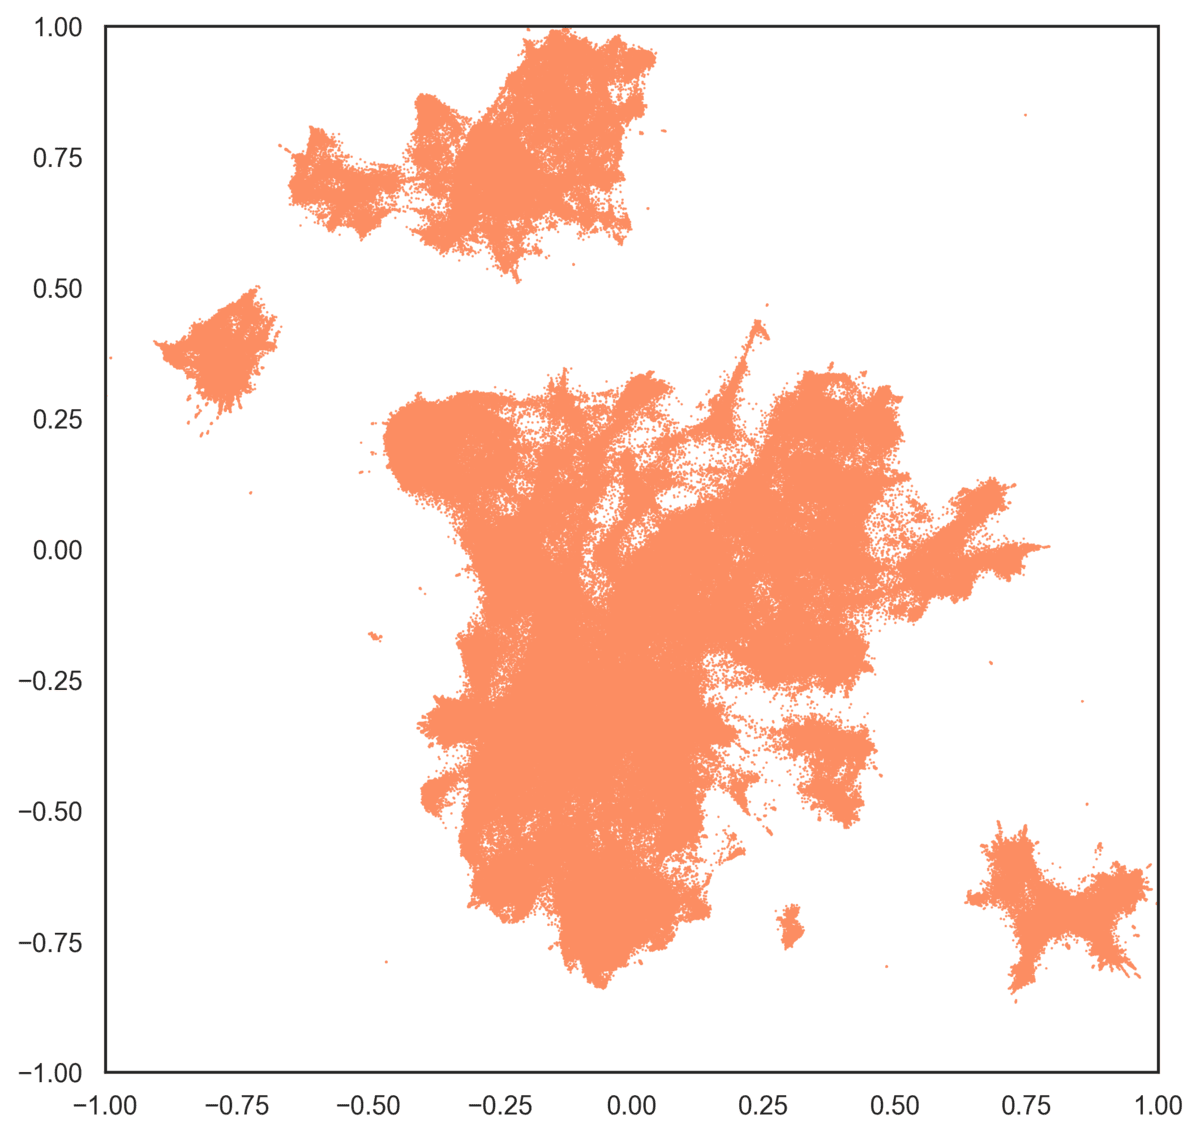
\includegraphics[width=.32\linewidth]{img/all-MiniLM-L6-v2_umap_1000000_20250912T171832.png}\label{fig:minilm-umap}}
    \hfill
    \subfigure[all-mpnet-base-v2 UMAP]{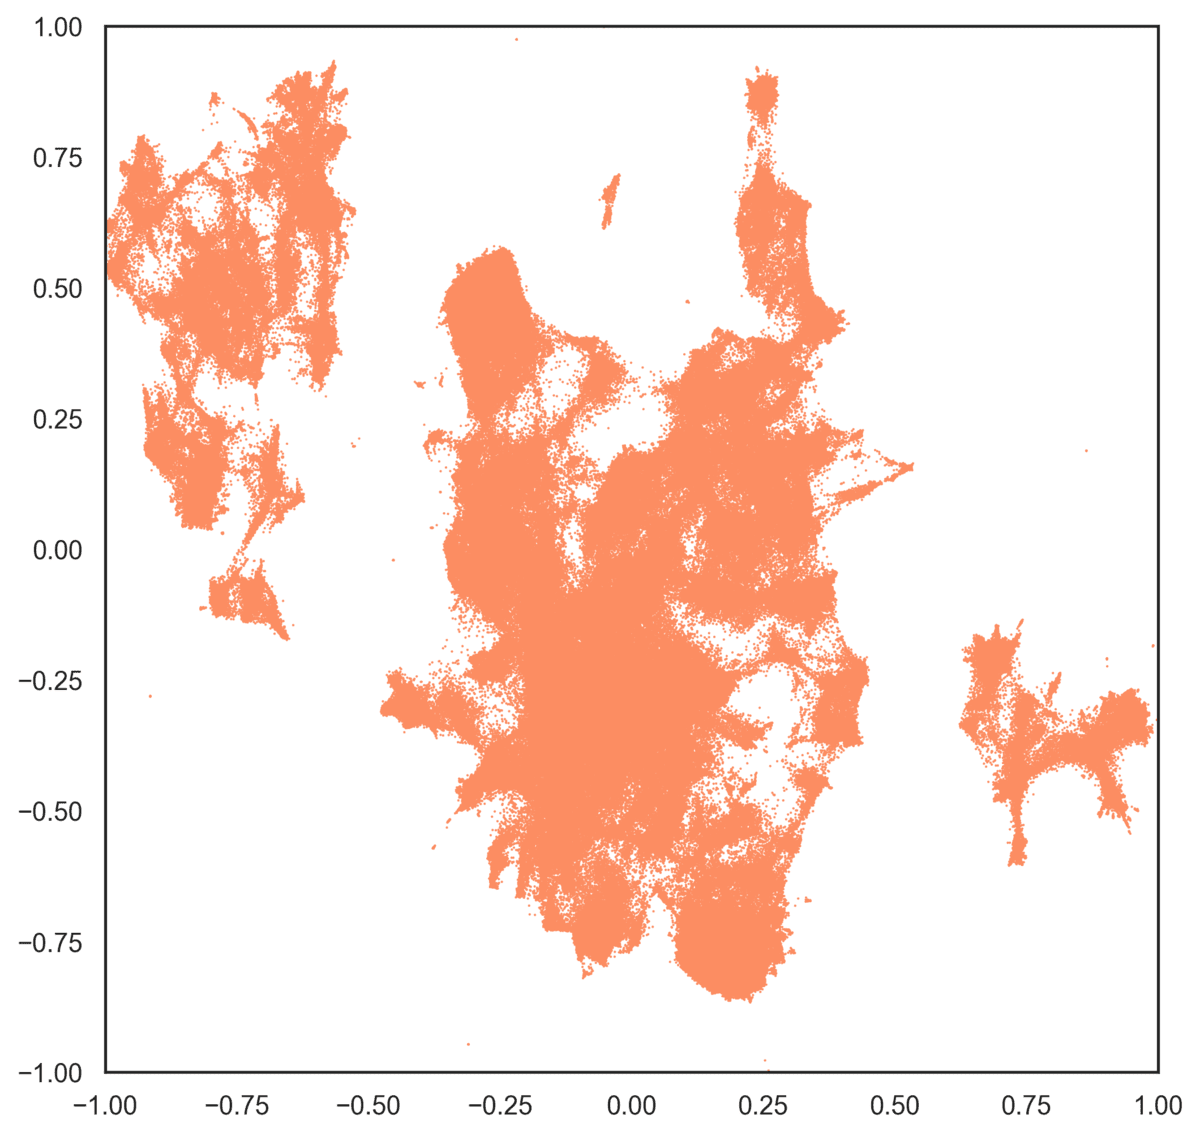
\includegraphics[width=.32\linewidth]{img/all-mpnet-base-v2_umap_1000000_20250912T171904.png}\label{fig:mpnet-umap}}
    \hfill
    \subfigure[nomic-embed UMAP]{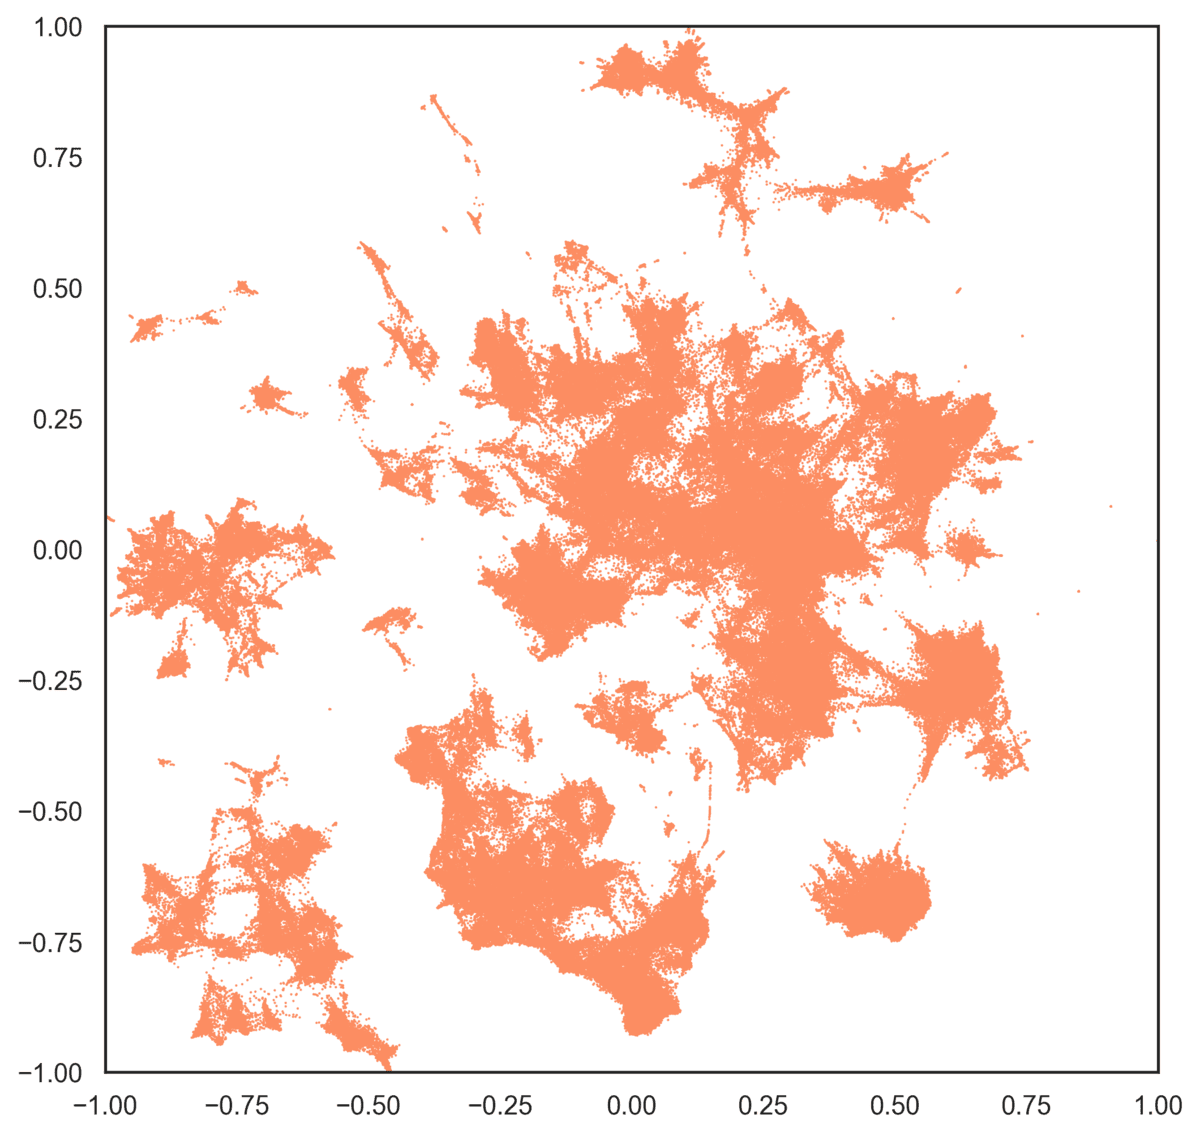
\includegraphics[width=.32\linewidth]{img/nomic-embed-text-v1.5_umap_1000000_20250912T171936.png}\label{fig:nomic-umap}}
    \caption{\label{fig:umap-comparison}
        Series of reduced embeddings using UMAP}
}

\maketitle
%-------------------------------------------------------------------------
\begin{abstract}
    Continual Learning can be computationally demanding, making on-device deployment challenging. In an effort to perform dimensionality reduction that can be dynamically adjusted based on user feedback and running on-device, this paper proposes a dataset generation pipeline, providing the foundation for such a model. With a subset of the Wikipedia dataset as a source, text embeddings are generated using pretrained models such as all-MiniLM-L6-v2, all-mpnet-base-v2 and nomic-embed-text-v1.5 \cite{nussbaumNomicEmbedTraining2025}. These high-dimensional vectors are then reduced to two-dimensional coordinates by applying UMAP and t-SNE. The resulting datasets are compared and analyzed regarding their visual legibility and spatial-semantic coherence. Alongside this paper, the generation pipeline and resulting datasets are published.
\end{abstract}

%-------------------------------------------------------------------------
%-------------------------------------------------------------------------
\section{Introduction}

The contemporary information landscape is both vast and inflationary. This is particularly evident in technology-related fields, where professionals must constantly update, learn, and organize information to maintain effectiveness. An increasingly large portion of this cognitive effort is being supplemented by generative machine learning models: In the 2024 Stack Overflow developer survey 63.2\% of respondents reported the usage of AI tools \cite{AI2024Stack}.

However, the centralized architecture through which these systems are typically deployed, diminishes user ownership and autonomy. This concern extends beyond mere convenience, as recent research also suggests cognitive implications: A study by Kosmyna et al. indicates that the use of ChatGPT for essay writing is associated with decreased neural connectivity and recall ability \cite{kosmynaYourBrainChatGPT2025}.

- assistance in knowledge organization instead of generation
- dimensionality reduction (DR)
- lack of stability upon database changes
- rerun on every addition
- multi stage pipeline with huge emebdding model not suitable for on-device continual learning

solution: small direct embedding model

How can sBERT embeddings combined with dimensionality reduction techniques like PCA, t-SNE, and UMAP be used to generate a training dataset that maps encyclopedic texts to spatial coordinates?

In response, this paper incorporates the following contributions:

\begin{itemize}
    \item A brief overview of available algorithms to perform dimensionality reduction of high-dimensional data (\ref{sec:rel-work})
    \item A reproducible pipeline for constructing datasets that map semantic embeddings to two-dimensional coordinates (\ref{sec:pipeline})
    \item A brief analysis and comparison of the data generated (\ref{sec:results})
\end{itemize}

%-------------------------------------------------------------------------
\section{Related Work}
\label{sec:rel-work}

A central challenge for continual learning on-device lies in computational overhead. Since both embedding generation and dimensionality reduction are required, two resource-intensive algorithms must be executed repeatedly, restricting feasibility in constrained environments.

Embedding generation is the prerequisite for understanding and comparing textual data. Sentence-BERT (sBERT) \cite{reimersSentenceBERTSentenceEmbeddings2019a} produces contextual embeddings that account for word order and surrounding semantics, making it a well-established foundation in many downstream natural language processing (NLP) tasks. In this work, sBERT serves as the primary framework to generate high-dimensional embeddings. However, these embeddings alone are not directly interpretable, requiring an additional DR step for visualization.

Dimensionality reduction techniques such as PCA, t-SNE, and UMAP are widely applied to high-dimensional data for visualization and interactive exploration \cite{smilkovEmbeddingProjectorInteractive2016}. PCA provides a stable linear reduction and is frequently used as a preprocessing step. t-SNE remains a popular choice for uncovering fine-grained local clusters but is computationally demanding. OpenTSNE implementations improve efficiency and scalability, making it more suitable for large datasets \cite{policarOpenTSNEModularPython2024}. UMAP, in contrast, emphasizes global structure while still preserving local neighborhoods \cite{mcinnesUMAPUniformManifold2020a}. This property makes UMAP complementary to t-SNE: While t-SNE excels at separating dense clusters, UMAP offers continuity across regions of semantic space.

Finally, commercial systems such as Nomic Atlas \cite{duderstadtAtlasWhitepaperScalable} adopt a similar approach, embedding large-scale corpora and projecting them into low-dimensional interactive maps. Atlas is designed for scalability and integrates with projection frameworks such as NOMAD \cite{nussbaumNomicEmbedTraining2025}. However, parts of the system remain proprietary, limiting reproducibility. In contrast, the dataset generation pipeline proposed here is aimed at small models suitable for continual learning while remaining fully open-source.

%-------------------------------------------------------------------------
\section{Dataset Generation from Dimensionality Reduction }
\label{sec:main}

This dataset is supposed to express similarity in content as spatial proximity between data points. The process is divided into two stages: First, the textual data is converted into a semantic text embeddings and secondly, the high-dimensional embedding vector is reduced to two dimensions.

%-------------------------------------------------------------------------
\subsection{Pipeline Implementation}
\label{sec:pipeline}

As a prerequisite, this paper assumes an existing source dataset of texts. Due to scope, size and availability the wikipedia dataset (20231101.en subset) was chosen \cite{WikimediaWikipediaDatasets2025}.

The proposed pipeline was developed and tested locally on a desktop workstation with the following specifications:
\begin{itemize}
    \item An Intel Core i9-10980XE CPU (3.00GHz)
    \item an NVIDIA Quadro RTX 5000 (16GB) GPU
    \item 128 GB RAM.
\end{itemize}

\begin{figure*}[htb]
    \centering
    \begin{tikzpicture}[
            scale=0.9,
            node distance=1.5cm and 2cm,
            box/.style={draw, rectangle, align=center, font=\small, inner sep=0.28cm}
        ]
        \node[box] (A) {wikipedia\\20231101.en};
        \node[box, right=of A] (B) {subset};
        \node[box, right=of B] (D) {sBERT\\embedding};
        \node[box, right=of D] (F) {PCA};

        \coordinate (split) at ($(F.east)+(2,0)$);

        \node[box, above=of split] (G) {tSNE};
        \node[box, below=of split] (H) {UMAP};

        \draw[->] (A) -- (B);
        \draw[->] (B) -- (D);
        \draw[->] (D) -- (F);

        \draw[->] (F.east) -- (split) -| (G.south);
        \draw[->] (F.east) -- (split) -| (H.north);
    \end{tikzpicture}
    \caption{Data generation pipeline: A subset of 1M entries is selected from the wikipedia dataset. For each sBERT model, the embedding is inferred and then reduced to 50 dimensions in the principal component analysis (PCA). Finally, all entries are reduced using both tSNE and UMAP separately.}
    \label{fig:pipeline}
\end{figure*}

%-------------------------------------------------------------------------
\subsection{Results}
\label{sec:results}

\begin{figure*}[htb]
    \centering
    \subfigure[all-MiniLM-L6-v2 t-SNE]{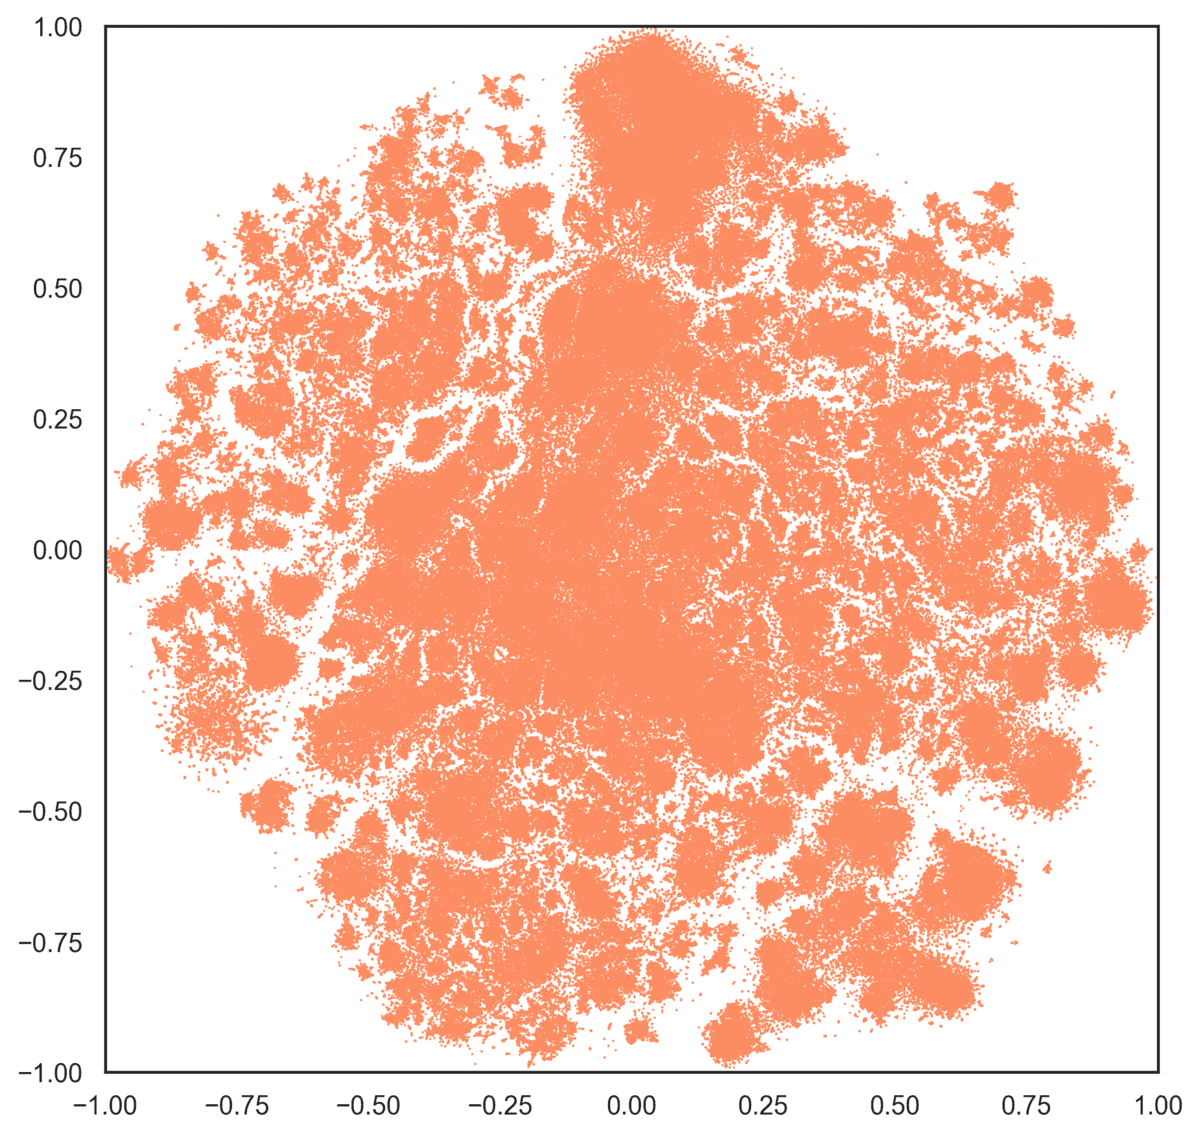
\includegraphics[width=.32\linewidth]{img/all-MiniLM-L6-v2_tsne_1000000_20250912T171816.png}\label{fig:minilm-tsne}}
    \hfill
    \subfigure[all-mpnet-base-v2 t-SNE]{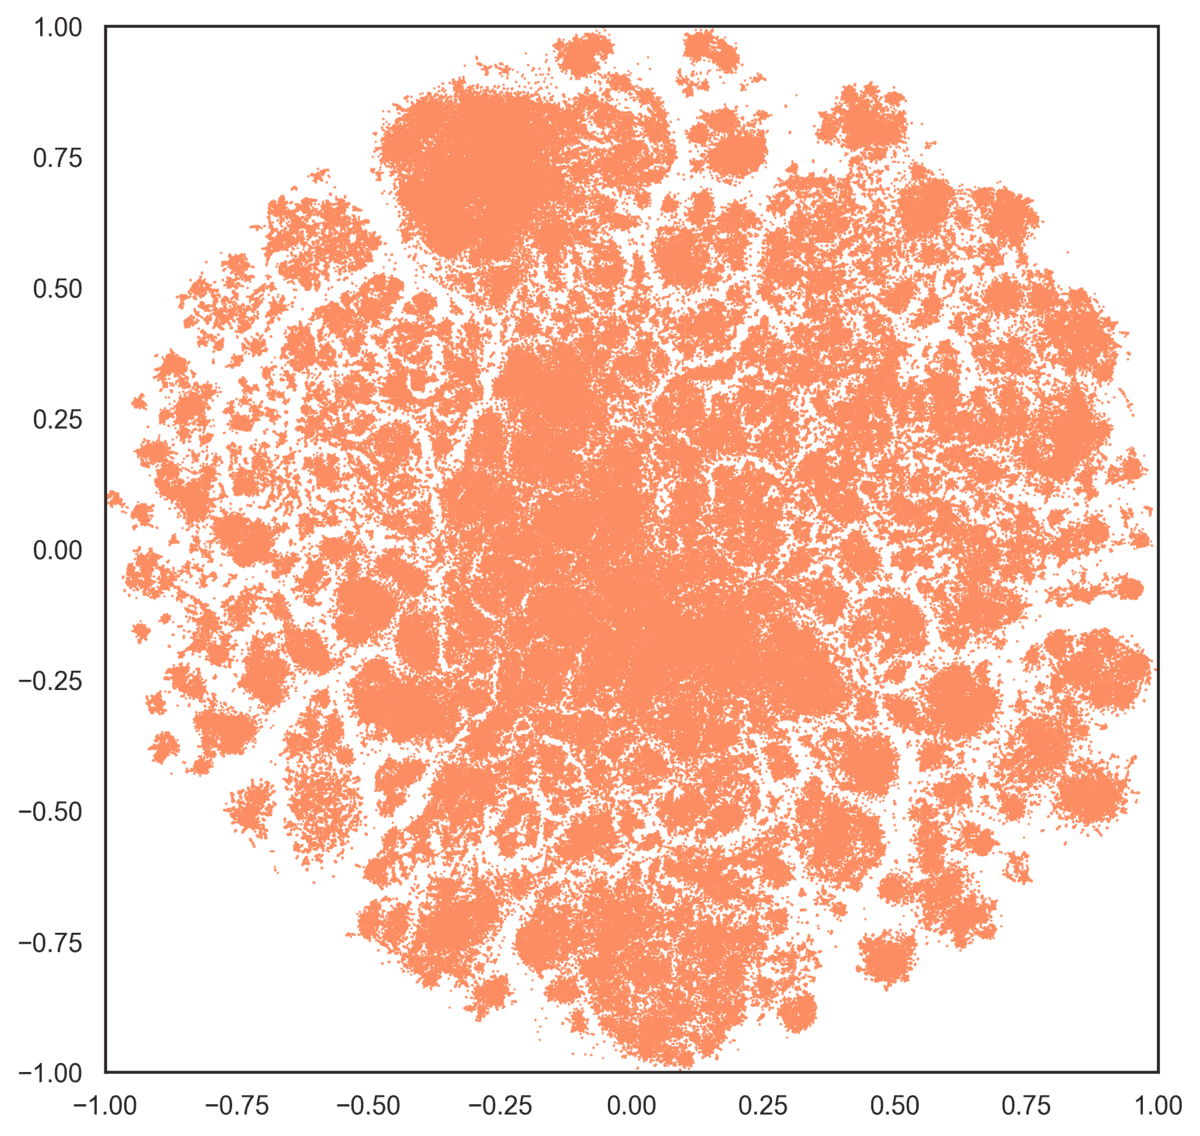
\includegraphics[width=.32\linewidth]{img/all-mpnet-base-v2_tsne_1000000_20250912T171848.png}\label{fig:mpnet-tsne}}
    \hfill
    \subfigure[nomic-embed t-SNE]{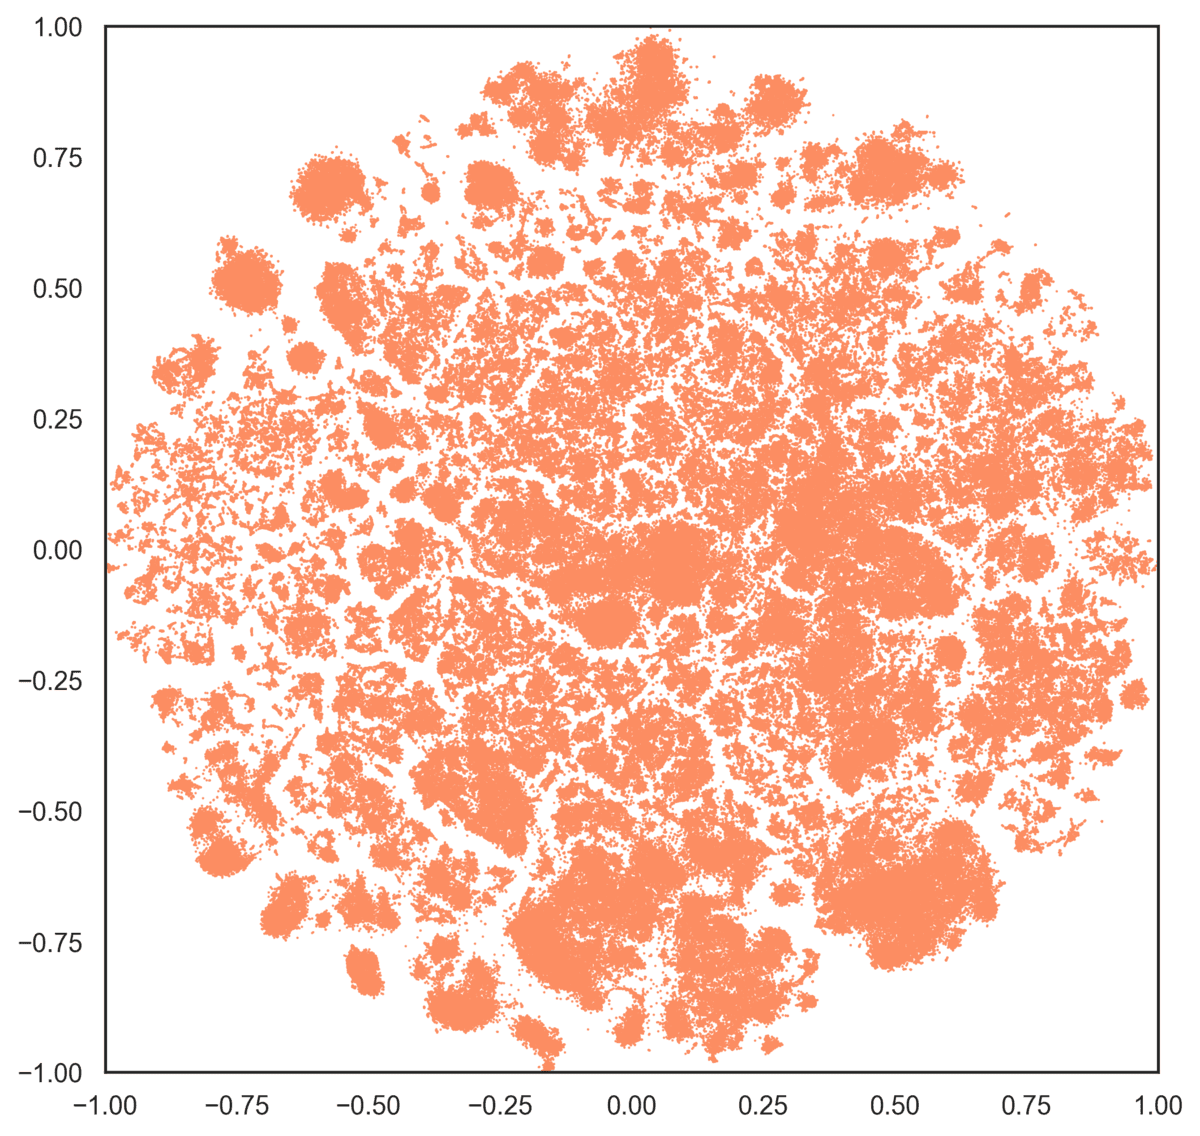
\includegraphics[width=.32\linewidth]{img/nomic-embed-text-v1.5_tsne_1000000_20250912T171920.png}\label{fig:nomic-tsne}}
    \caption{\label{fig:tsne-comparison}
        Series of reduced embeddings using t-SNE}
\end{figure*}

- dataset generated
- \autoref{fig:umap-comparison} and \autoref{fig:tsne-comparison} -> UMAP very pronounced global strucutes (landscape like), t-SNE better utilization of space

! table with times it took for generation

%-------------------------------------------------------------------------
\subsection{Evaluation}
\label{sec:eval}

- choice of dr -> choice of taste (space utilization vs global recognizability)
- context length for embedding (Nomic embed only model that captures full articles others are truncated)

%-------------------------------------------------------------------------
\subsection{Discussion}
\label{sec:discussion}

- see umap or opentsne criqitue to usability of coords
- data domain specificity

%-------------------------------------------------------------------------
\section{Conclusion / Future Work}
\label{sec:conclusion}

- training of an actual model
- consideration of other dim reduction approaches (such as PaCMAP \cite{JMLR:v22:20-1061})

%-------------------------------------------------------------------------
\section{Data Availability}
\label{sec:data-av}

The source data used in this paper is the wikipedia dataset \cite{WikimediaWikipediaDatasets2025}, available on Huggingface (linked \href{https://huggingface.co/datasets/wikimedia/wikipedia}{here}). The resulting dataset generated using the described pipeline is also available on Huggingface (linked \href{https://huggingface.co/datasets/whatphiliptrains/wikipos}{here}).

%-------------------------------------------------------------------------
\section{Code Availability}
\label{sec:code-av}

The code for the described pipeline alongside the generation of the figures used in this paper is available on GitHub (linked \href{https://github.com/whatphilipcodes/wikipos}{here}).

%-------------------------------------------------------------------------

%\bibliographystyle{eg-alpha}
\bibliographystyle{eg-alpha-doi}

% FILMUNI: Add your own bib file here or
%  add your references to acsfubbib.bib
\bibliography{acsfubbib}

%-------------------------------------------------------------------------


\end{document}
